\section{Diseño e implementación}
\subsection{Productos ejecutables}
	\begin{frame}{Productos ejecutables}
		\begin{enumerate}
		 	\item Rutinas automatizadas: se ejecutan a partir del entorno gráfico del sistema operativo.
		 	\item Portal de usuario: se ofrece como una página web, la cual depende del servidor web de la farmacéutica y del explorador web del usuario.
		\end{enumerate}
	\end{frame}
	\begin{frame}{Automatización de rutinas}
		\begin{figure}[h]
		\centering
		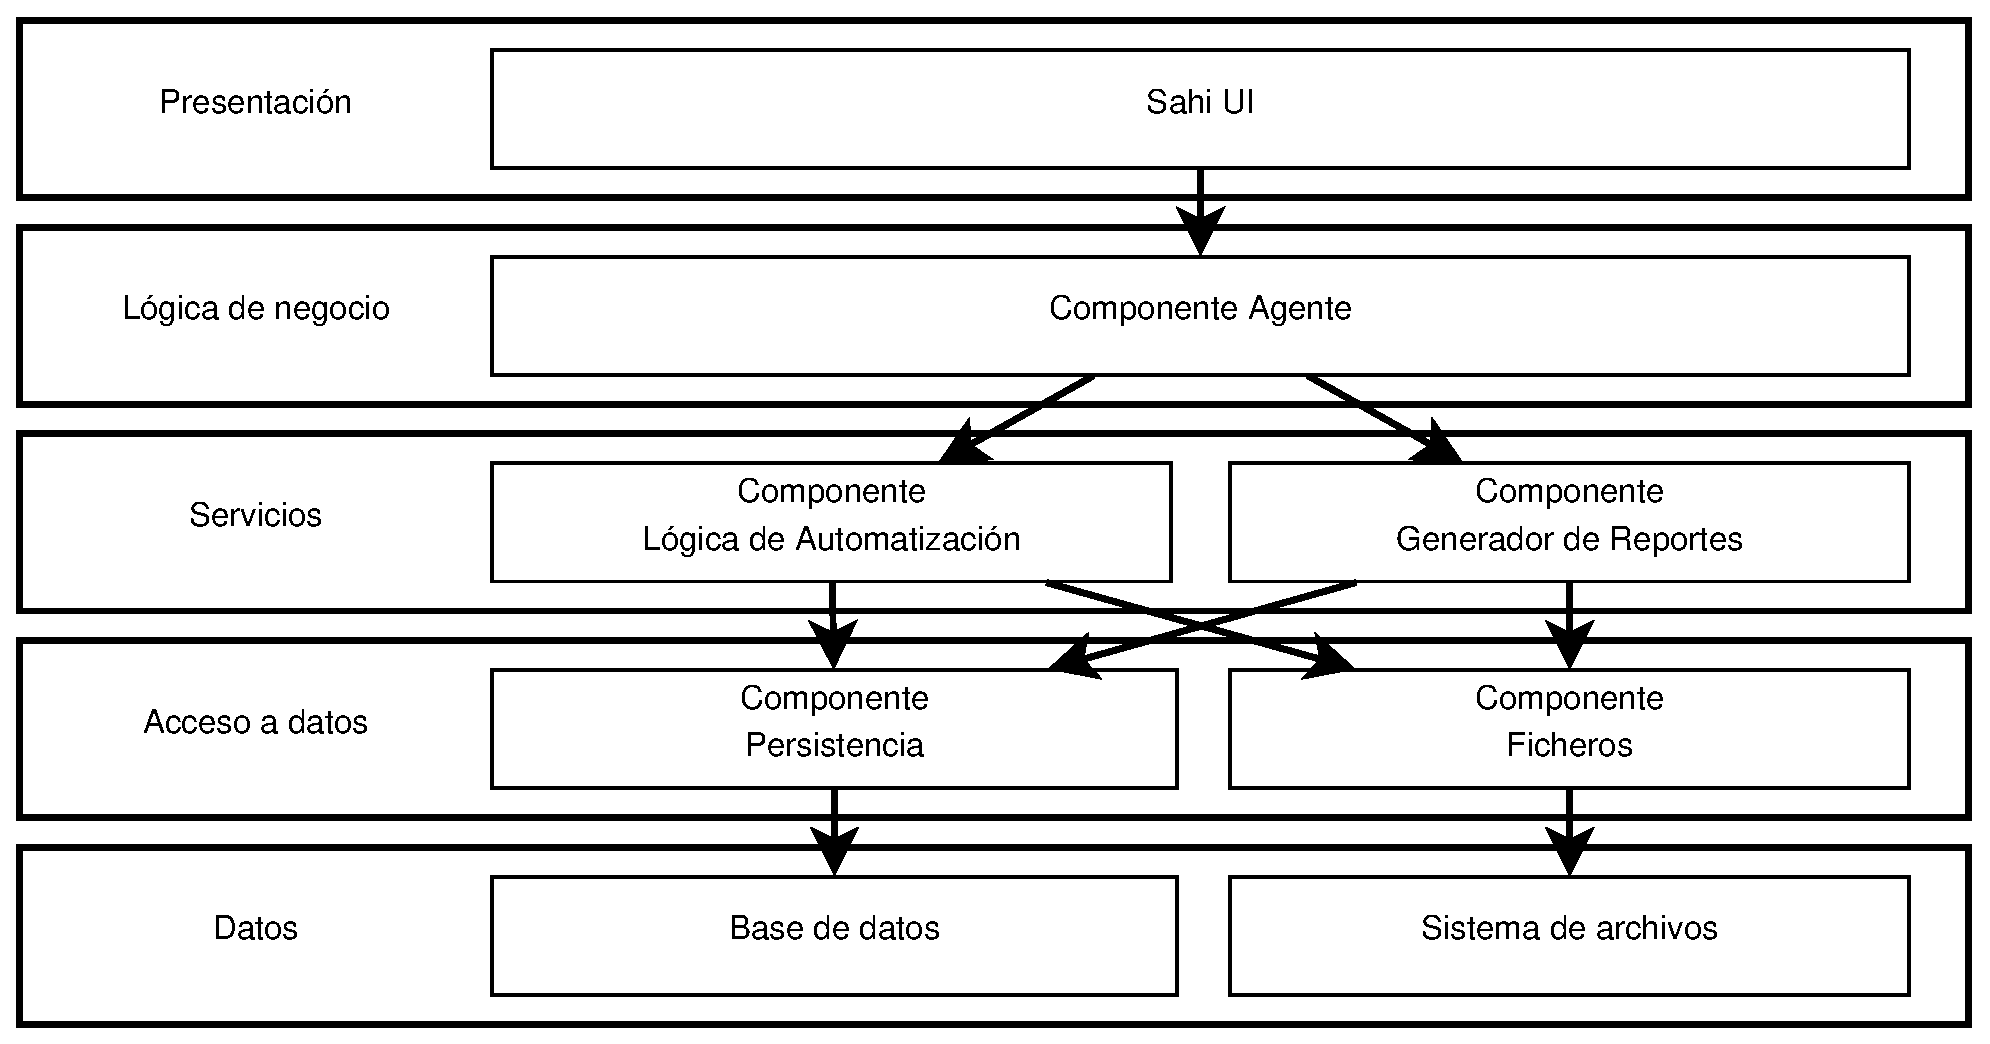
\includegraphics[width=\textwidth]{dia-layers-auto}
		\label{fig:dia-layers-auto}
		\end{figure}
	\end{frame}
	\begin{frame}{Aplicación web}
		\begin{figure}[h]
		\centering
		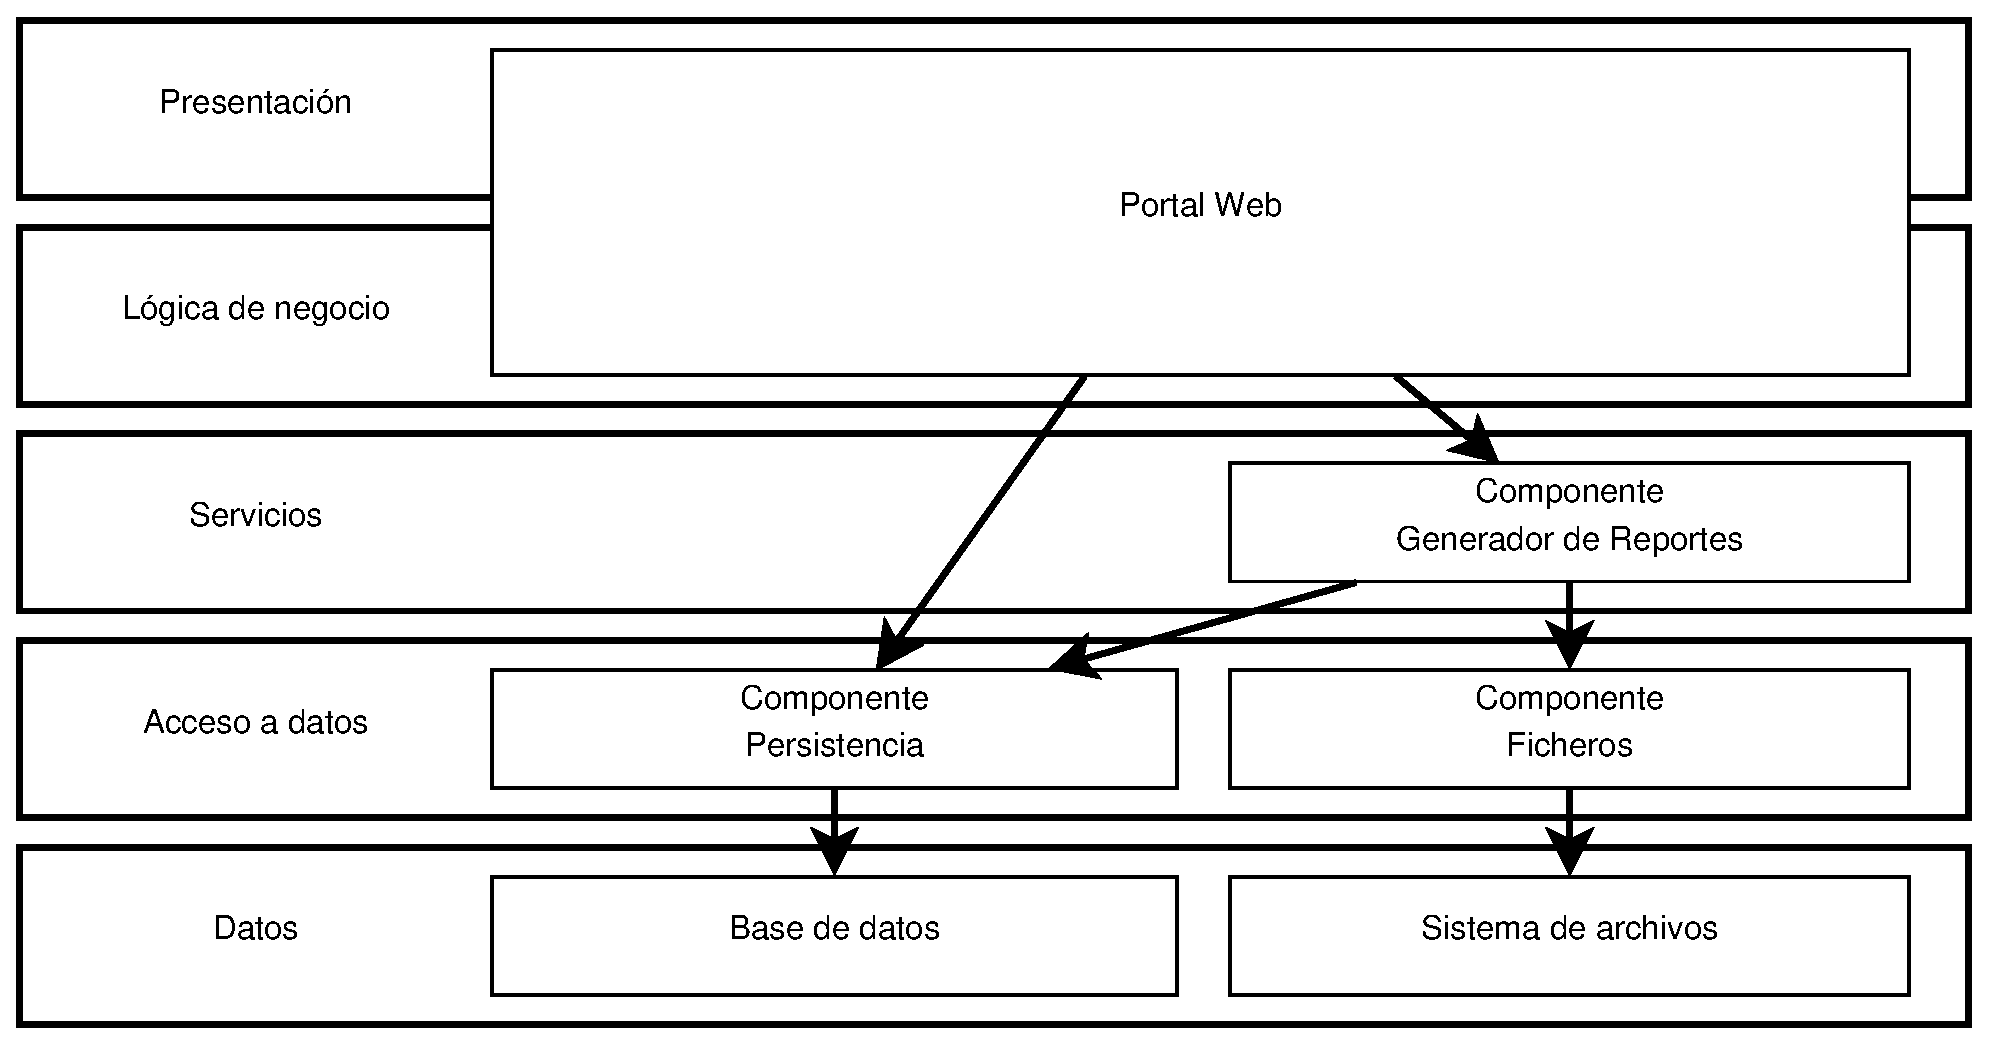
\includegraphics[width=\textwidth]{dia-layers-web}
		\label{fig:dia-layers-web}
		\end{figure}
	\end{frame}

\subsection{Componentes de AutoSA}
	\begin{frame}{Componentes de AutoSA}
		\centering
		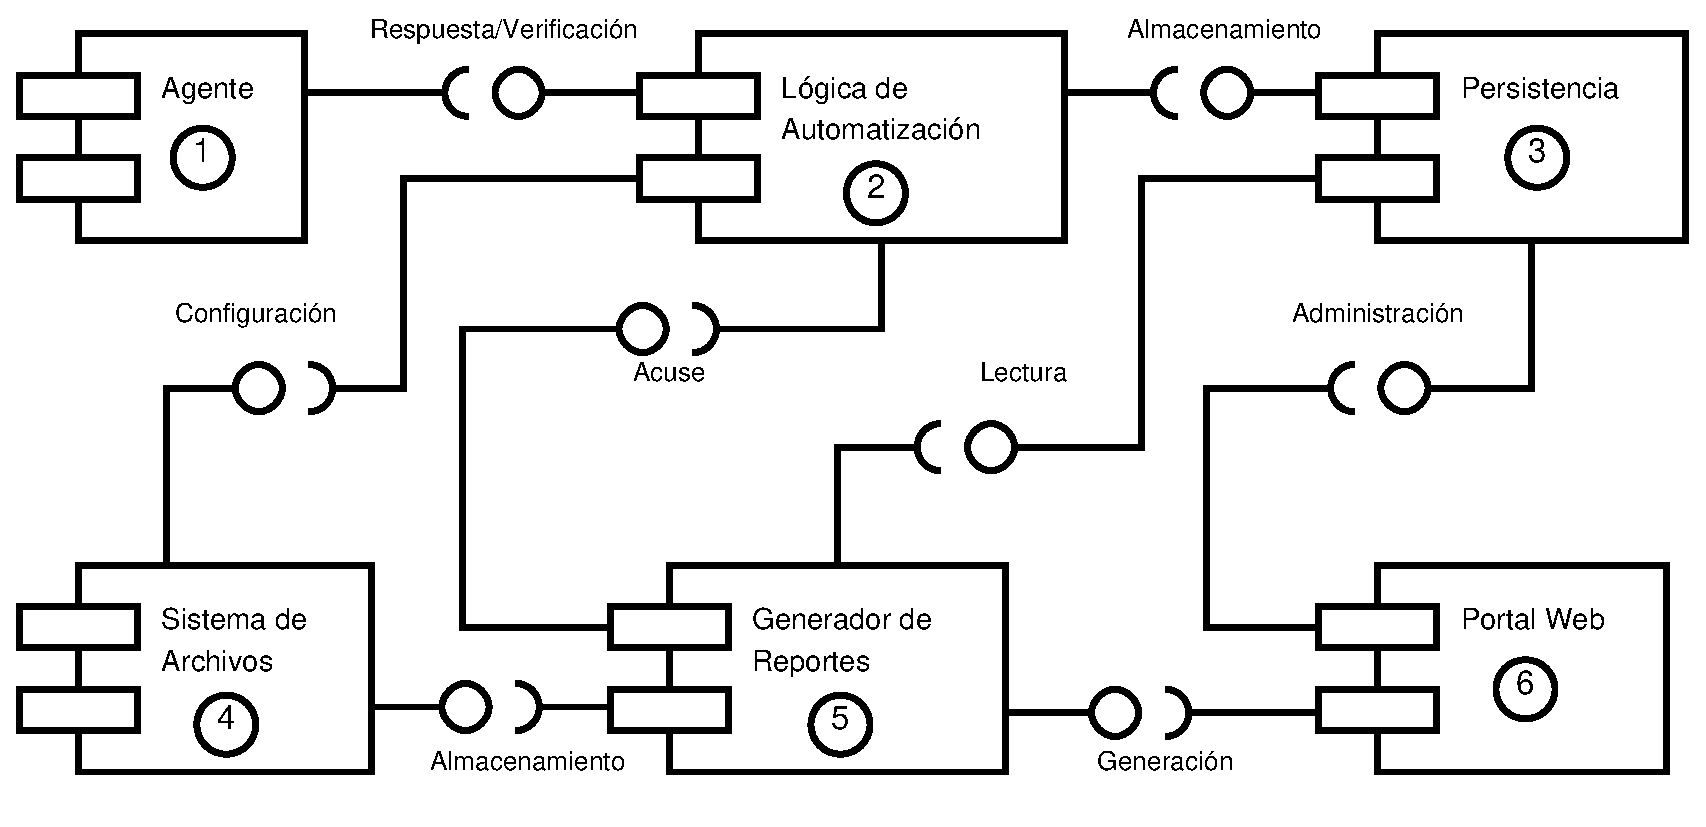
\includegraphics[width=\textwidth]{dia-components}
	\end{frame}

\subsection{Diagrama de paquetes}
	\begin{frame}{Diagrama de paquetes}
		\centering
		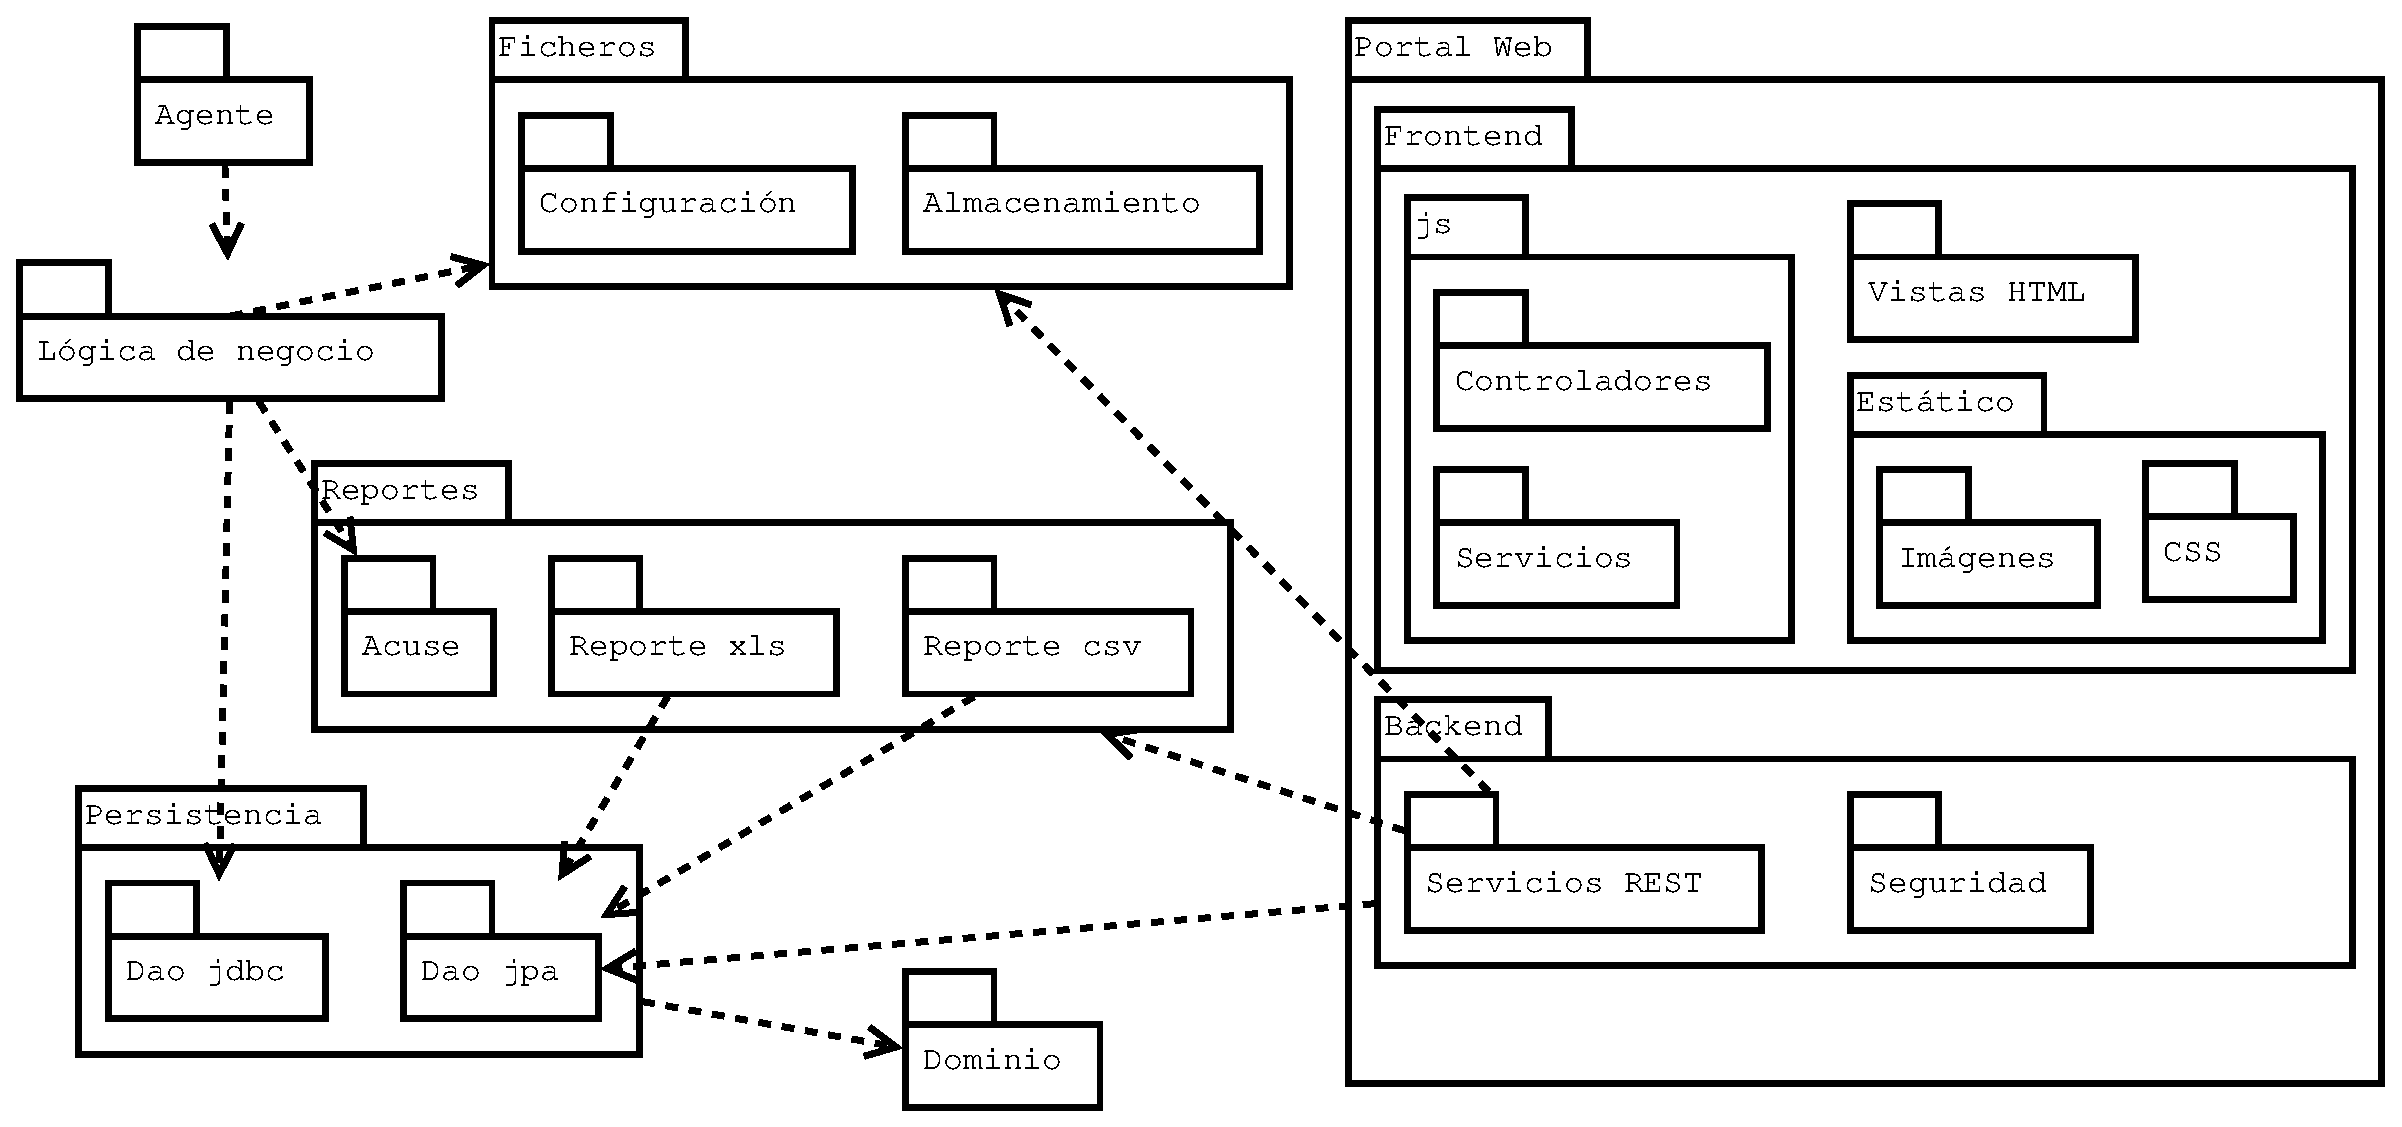
\includegraphics[width=\textwidth]{dia-package-large}
	\end{frame}
